
\chapter*{ಅನುಬಂಧ : III}

\section*{ತಾಯಿತಗಳಲ್ಲಿ ಮಾಯಾಚೌಕ :}

ಮಾಯಾಚೌಕವು ಆವಿಷ್ಕಾರವಾದ ಮೊದಲ ದಿನಗಳಲ್ಲಿ ಮಾನವ ಅದರ ವಿಶಿಷ್ಟತೆ ಹಾಗೂ \linebreak ವೈಚಿತ್ರ್ಯವನ್ನು ಕಂಡು ಚಕಿತನಾದ. ಅಡ್ಡಸಾಲು, ಕಂಭಸಾಲು ಮತ್ತು ಕರ್ಣಗಳ ಸಂಖ್ಯೆಗಳು ಒಂದೇ ಮೊತ್ತವನ್ನು ನೀಡುವುದು ಅವನನ್ನು ವಿಸ್ಮಯಗೊಳಿಸಿತು. ಇದರಿಂದಾಗಿ ಮಾಯಾ\-ಚೌಕಗಳಿಗೆ ಅಲೌಕಿಕ ಶಕ್ತಿ ಇದೆಯೆಂದು ಆರೋಪಿಸಿದ. ಈ ಶಕ್ತಿಯಿರುವ ಮಾಯಾಚೌಕವನ್ನು ತಾಯಿತವಾಗಿ ಮಾಡಿ ಧರಿಸಿದರೆ ರೋಗಗಳು ವಾಸಿಯಾಗುವುವು, ಕಳ್ಳಕಾಕರ, ಬೆಂಕಿಯ ಉಪದ್ರವಗಳಿಂದ ಪಾರಾಗಬಹುದು ಎನ್ನುವ ನಂಬಿಕೆ ಬಂದು ಮಾಯಾಚೌಕಗಳ ತಾಯಿತಗಳನ್ನು ಧರಿಸುವ ಪ್ರವೃತ್ತಿ ಬೆಳೆಯಿತು. ಯೂರೋಪ್, ಇಸ್ಲಾಮಿಕ್ ರಾಷ್ಟ್ರಗಳು, ಮತ್ತು ಭಾರತ ಇವುಗಳಲ್ಲಿ ತಾಯಿತದ ಬಳಕೆ ಗಣನೀಯವಾಗಿ ಕಂಡುಬಂದಿತು. ಇಂದೂ ಸಹ ಹಲವರು ತಾಯಿತ ಅಥವಾ ರಕ್ಷೆಗಳಿಗೆ ಮೊರೆ ಹೋಗುವುದನ್ನು ಕಾಣಬಹುದು.

ಮಾಯಾಚೌಕಗಳ ತಾಯಿತ / ರಕ್ಷೆಗಳಿಗೆ ವಿಶೇಷ ಅಲೌಕಿಕ ಶಕ್ತಿ ಇದೆ ಎನ್ನುವುದಕ್ಕೆ ಯಾವುದೇ ವೈಜ್ಞಾನಿಕ ಆಧಾರ ಕಂಡುಬಂದಿಲ್ಲ. ಸಂಖ್ಯೆಗಳ ಜೋಡಣೆಗೂ ಭೌತ ಪ್ರಪಂಚದಲ್ಲಿ ಅವು ಬೀರಬಹುದೆನ್ನಲಾದ ಪ್ರಭಾವಗಳಿಗೂ ಇರಬಹುದಾದ ಸಂಬಂಧವನ್ನು ಕುರಿತು ಪ್ರಯೋಗ/ ಪರೀಕ್ಷೆಗಳಿಂದ ನಿರ್ಧರಿಸಿಲ್ಲ. ಯಾವುದೇ ಶಾಸ್ತ್ರ ಸಿದ್ಧಿಯಾಗಲೀ, ಸಿದ್ಧಶಾಸ್ತ್ರವಾಗಲೀ ಇಲ್ಲ. ಇದು ಕೇವಲ ‘‘ಮೂಢನಂಬಿಕೆ’’ ಎನ್ನಲಾಗಿದೆ.

ಈ ಕೆಳಗೆ ತಾಯಿತ/ರಕ್ಷೆಗಳ ಕೆಲವು ಉದಾಹರಣೆಗಳನ್ನು ಕೊಡಲಾಗಿದೆ. ಇವು ಉಂಟು ಮಾಡುತ್ತವೆನ್ನಲಾದ ಪ್ರಭಾವಗಳಿಗೆ ಯಾವುದೇ ವೈಜ್ಞಾನಿಕ ಆಧಾರವಾಗಲೀ, ಶಾಸ್ತ್ರೀಯ ಸಿದ್ಧಿಯಾಗಲೀ, ಇಲ್ಲವೆನ್ನುವುದನ್ನು ಮತ್ತೊಮ್ಮೆ ನೆನಪಿಸಬೇಕಾಗಿದೆ.

ಅರಬ್ಬರು ಮಾಯಾಚೌಕ ತಾಯಿತಗಳ ಶಕ್ತಿಯ ಬಗ್ಗೆ ಬಹಳ ನಂಬಿಕೆ ಇರಿಸಿದ್ದರು. \hbox{ಕೆಲವು} ತಾಯಿತಗಳನ್ನು ಅಂಗವಿಕಲರ ರಕ್ಷಣೆಗೆಂದು ಬಳಸುತ್ತಿದ್ದರು. ಮತ್ತೆ ಹಲವು \hbox{ತಾಯಿತಗಳನ್ನು} ಪ್ರಸವ ವೇದನೆಗೆ ಇರುವ ಗರ್ಭಿಣಿಯರಿಗೆ ತೋರಿಸಿ, ಹೊಟ್ಟೆಯ ಮೇಲೆ ಅದನ್ನಿರಿ\-ಸಿದರೆ \hbox{ಸುಖಪ್ರಸವವಾಗುವುದೆಂದು} ಭಾವಿಸಿದ್ದರು. ಸೈನಿಕರು ತೊಡುತ್ತಿದ್ದ ಅಂಗಿಯ ಮೇಲೆ ಮಾಯಾ\-ಚೌಕವನ್ನು ಕಸೂತಿ ಹಾಕಿದರೆ ಅವರಿಗೆ ರಕ್ಷಣೆ ದೊರೆಕುವುದೆಂಬ ನಂಬಿಕೆ ಇದ್ದಿತು. ಈ ಕೆಳಗೆ ಕೊಟ್ಟಿರುವ ತಾಯಿತದ 2 ಮಾದರಿ ನೋಡಿ.
\begin{figure}[H]
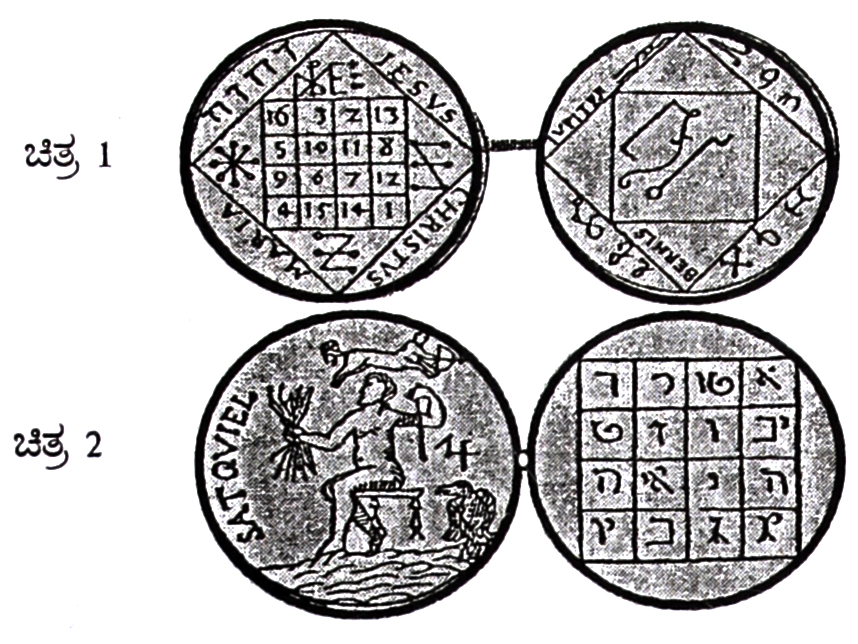
\includegraphics[scale=1.2]{src/figures/chap11/fig11-1.jpg}
\end{figure}

ಕ್ರಿಶ್ಚಿಯನ್ನರಲ್ಲಿಯೂ ತಾಯಿತ/ರಕ್ಷೆಯ ನಂಬಿಕೆ ಇದ್ದುದು ತಿಳಿದು ಬಂದಿದೆ. ಕೆಳಗಿನ \linebreak ಎರಡು ಉದಾಹರಣೆಗಳನ್ನು ಗಮನಿಸಿ. ಒಂದು ಗುರುಗ್ರಹದ ತಾಯಿತ. ಇದರ ಒಂದು ಬದಿಯಲ್ಲಿ 34 ಮೊತ್ತದ $4 \times 4$ ಮಾಯಾಚೌಕವಿದೆ. ಗುರುಗ್ರಹ ಉಚ್ಚಸ್ಥಿತಿಯಲ್ಲಿರುವ ಕಾಲದಲ್ಲಿ ಬೆಳ್ಳಿಯ ತಗಡಿನಲ್ಲಿ ಈ ಚೌಕವನ್ನು ಕೆತ್ತಿಸಿ, ಧರಿಸಿದರೆ ಐಶ್ವರ್ಯ, ಸುಖ, ಶಾಂತಿ ಲಭಿಸುತ್ತದೆಂಬ ನಂಬಿಕೆ.

\medskip
ಇನ್ನೊಂದು ಮಂಗಳ ಗ್ರಹದ ತಾಯಿತ. ಇದರ ಒಂದು ಬದಿಯಲ್ಲಿ ಚೌಕದ 65 \linebreak ಮೊತ್ತವಿದೆ. ಮಂಗಳ ಗ್ರಹ ಉಚ್ಛಸ್ಥಿತಿಯಲ್ಲಿರುವ ಕಾಲದಲ್ಲಿ ಈ ಚೌಕ ಮತ್ತು ಆಕೃತಿಯನ್ನು \linebreak ಕಬ್ಬಿಣದ ಹಾಳೆಯ ಮೇಲೆ ಕೆತ್ತಿಸಿ, ಧರಿಸಿದರೆ ನ್ಯಾಯಾಲಯ ವಿವಾದಗಳಲ್ಲಿ ಜಯ ಸಿಗುವುದೆಂದು ನಂಬಿಕೆ. ಖಡ್ಗದ ಮೇಲೆ ಇದನ್ನು ಕೆತ್ತಿಸಿ ಬಳಸಿದಾಗ ಶತ್ರು ನಿರ್ಮೂಲನ ಶಕ್ತಿ ಬರುವುದೆಂದು ಕಲ್ಪಿಸಲಾಗಿತ್ತು.

\begin{figure}[H]
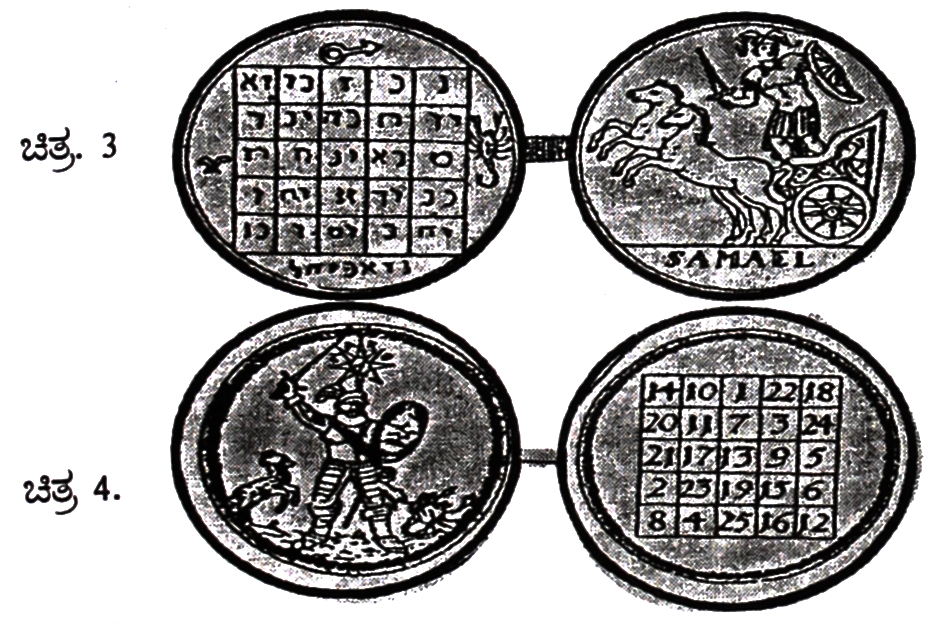
\includegraphics{src/figures/chap11/fig11-2.jpg}
\end{figure}

ಭಾರತದಲ್ಲಿಯೂ ಈ ತಾಯಿತ ಪರಂಪರೆ ಕಂಡುಬರುತ್ತದೆ. ಮಾನವರಿರುವೆಲ್ಲೆಡೆ \linebreak ಮೂಢನಂಬಿಕೆಯೂ ಜೊತೆ ಜೊತೆಯಾಗಿರುವುದಲ್ಲವೆ? ಮಕ್ಕಳ ಜ್ವರ ನಿವಾರಣೆಗೆಂದು ಬಳಸುತ್ತಿದ್ದ ಒಂದು ತಾಯಿತ ಹೀಗಿದೆ. ಪಂಚಲೋಹದ ತಗಡಿನಲ್ಲಿ ಈ ಮಾಯಾಚೌಕವನ್ನು ಬರೆದು, ಸ್ವಲ್ಪ ಗೋರೋಜಿನ ಕಸ್ತೂರಿ ಹಾಕಿ ಅಷ್ಟ ವಿಧಾನಾರ್ಚನೆಯಿಂದ ಪೂಜಿಸಿ, ಬೆಳ್ಳಿ ಕೊಳವೆಯಲ್ಲಿ ಹಾಕಿ ಮಕ್ಕಳ ಕತ್ತಿಗೆ ಕಟ್ಟಿದರೆ ಯಾವ ವಿಧದ ಜ್ವರವೂ ನಿವಾರಣೆಯಾಗುತ್ತದೆಂಬ ನಂಬಿಕೆ. 22 ಮೊತ್ತದ ಈ ಮಾಯಾಚೌಕ ವಿಶಿಷ್ಟ ರೀತಿಯಲ್ಲಿ ಅದೇ ಮೊತ್ತ ಕೊಡುವುದನ್ನು ಗಮನಿಸಿ.
\begin{figure}[H]
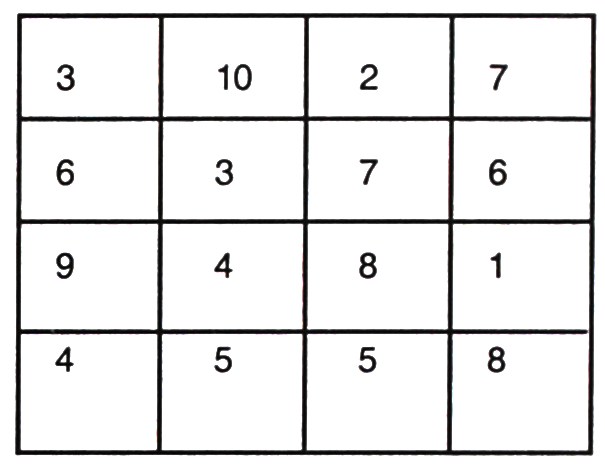
\includegraphics{src/figures/chap11/fig11-3.jpg}
\end{figure}

ಮತ್ತೊಂದು ಉದಾಹರಣೆ ನೋಡಿ

ಈ ಮಾಯಾಚೌಕವನ್ನು (ಅದಕ್ಕೆ ಯಂತ್ರ ಎಂಬ ಹೆಸರು) ಲೋಹದ ತಗಡಿನಲ್ಲಿ \hbox{ಬರೆದು} ಭುಜಪತ್ರೆ ನವಾಸಾರಗಳನ್ನು ಹಾಕಿ ಪೂಜಿಸಿ ಮಗುವಿನ ಕೊರಳಿಗೆ ಕಟ್ಟಿದರೆ ಸರ್ವಭಯ \linebreak ನಿವಾರಣೆಯಾಗುತ್ತದೆ ಎಂಬ ನಂಬಿಕೆ.
\begin{figure}[H]
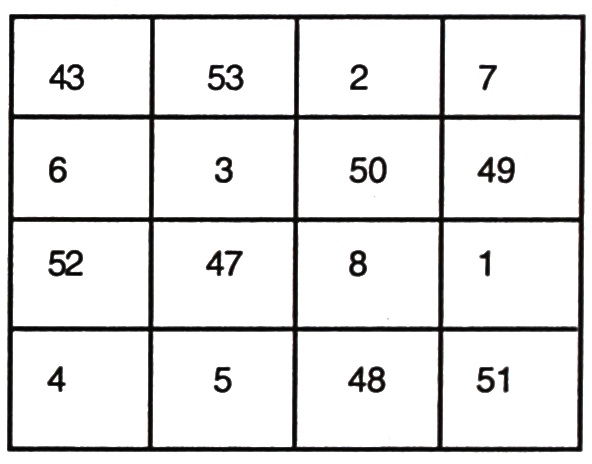
\includegraphics{src/figures/chap11/fig11-4.jpg}
\end{figure}

108 ಮೊತ್ತದ ಈ ಮಾಯಾಚೌಕ ಸಾಧಾರಣ ಚೌಕ ಅಷ್ಟೇ.

ಇವೇ ಅಲ್ಲದೇ ಇನ್ನೂ ಅನೇಕ ಯಂತ್ರ (ಮಾಯಾಚೌಕದ ತಾಯಿತ) ಗಳ ಉದಾಹರಣೆ ಇವೆ. ಹೊಲದ ರಕ್ಷಣೆಗೆ, ಪಶುಗಳ ದೃಷ್ಟಿನಿವಾರಣೆಗೆ, ಪ್ರಸವ ವೇದನೆ ಶಮನಕ್ಕೆ, ಕಾರ್ಯ\-ದಲ್ಲಿ  ಜಯಗಳಿಸಲು, ಚೋರ ಭಯನಿವಾರಣೆಗೆ, ಮಕ್ಕಳ ದೃಷ್ಟಿದೋಷ ನಿವಾರಣೆಗೆ, ಇತ್ಯಾದಿ\-ಗಳಿಗೆ ವಿವಿಧ ಮಾಯಾಚೌಕಗಳ ತಾಯಿತಗಳನ್ನು ವಿಶಿಷ್ಟ ರೀತಿಯಲ್ಲಿ ತಯಾರಿಸಿ, ಬಳಸುವ ಪದ್ಧತಿ\-ಗಳು ಇವೆ.

ಇಷ್ಟಾದರೂ ಒಂದು ಅಂಶ ಗಮನದಲ್ಲಿರಲಿ. ತಾಯಿತಗಳ ಬಳಕೆಗೆ ಯಾವುದೇ \hbox{ವೈಜ್ಞಾನಿಕ ಆಧಾರವಿಲ್ಲ.} ಪ್ರಯೋಗ ನಡೆಸಿ ಅವುಗಳ ಪರಿಣಾಮವನ್ನು ಒರೆ ಹಚ್ಚಿಯೂ ಇಲ್ಲ. ಕೆಲವೊಮ್ಮೆ \textbf{‘‘ಶ್ರದ್ಧಾ ನಿದಾನ’’} (faith cure)ದಿಂದ ಫಲ ಸಿಕ್ಕಿರಬಹುದು. ಇದು \hbox{ತಾಯಿತದ} ಶಕ್ತಿ ಎನ್ನುವುದು ಕಾಕತಾಳೀಯವಷ್ಟೇ. ಈ ದಿನಗಳಲ್ಲೂ ಹಲವಾರು ಸುಶಿಕ್ಷತರೂ ಈ \hbox{ತಾಯಿತ/ರಕ್ಷೆ} ಧರಿಸುತ್ತಿರುವುದು ದುರದೃಷ್ಟಕರ !
\begin{center}
*****
\end{center}

\begin{figure}[H]
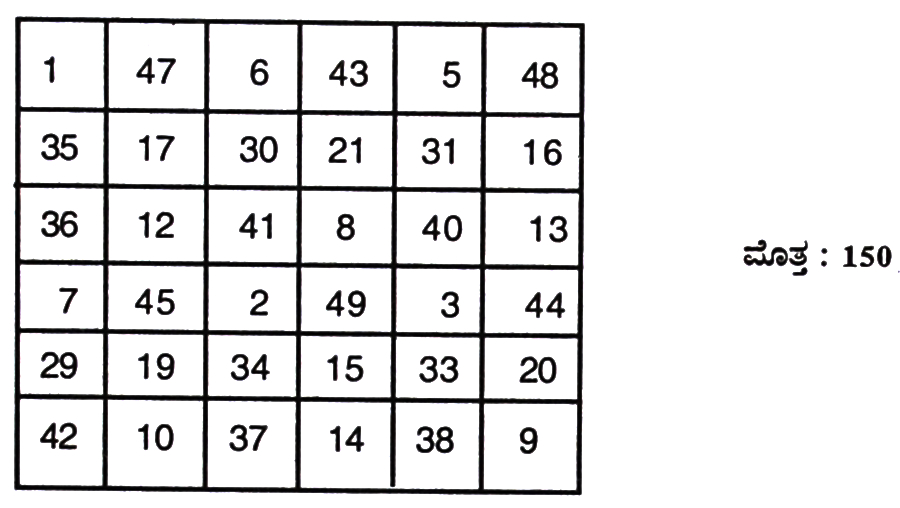
\includegraphics{src/figures/chap11/fig11-5.jpg}
\end{figure}
\begin{itemize}
	\item ಸಂಖ್ಯೆಗಳು ಕ್ರಮಾಗತವಾಗಿಲ್ಲ.\smallskip
	\item ಮೊತ್ತವನ್ನು ವರ್ಗ ಸೂಚಕ ಸಂಖ್ಯೆಯಿಂದ ಭಾಗಿಸಿದಾಗ $150 \div 6  = 25$\smallskip
	\item ಯಾವುದೇ $2^2 (2 \times 2)$ 
	
	ಚೌಕದ ಮನೆಗಳ ಸಂಖ್ಯೆಗಳ ಮೊತ್ತ $100 (4 \times 25 = 100)$\smallskip
	\item ಯಾವುದೇ $3^2 (3 \times 3)$ 
	
	ಚೌಕದ ಮನೆಗಳ ಸಂಖ್ಯೆಗಳ ಮೊತ್ತ $225 (9 \times 25 = 225)$\smallskip
	\item ಯಾವುದೇ $4^2 (4 \times 4)$ 
	
	ಚೌಕದ ಮನೆಗಳ ಸಂಖ್ಯೆಗಳ ಮೊತ್ತ $400 (16 \times 25 = 400)$\smallskip
\end{itemize}
\begin{center}
*****
\end{center}
